\documentclass[twocolumn]{article}

\usepackage[margin=1in]{geometry}
\usepackage{graphicx}
\usepackage{amssymb}
\usepackage{amsmath}

\title{Analysis: So Far}
\date{\today}

\begin{document}

\maketitle

\section{What's New}

\textbf{Basic idea \#1} is the straightforward observation that when looking for time series changepoints, we actually know exactly where to look - the time when the config change occurred. Previously, I was computing changepoints of each time series and attempting to use some window after a config change to find ``related'' changes. This is a bit clumsy: we don't have an indication of the ``magnitude'' of the change.

Looking slightly deeper at changepoint detection algorithms, it turns out some first compute a probability of a changepoint at each timestep, then pick points from the resulting time series (e.g., by thresholding). That is, for each metric, we can compute $P_{\textit{commit},\textit{node},\textit{metric}}$. Currently, it is summed over a window, which may or may not make sense depending upon the test.

\textbf{Basic idea \#2} is a heuristic: if a time series change is indeed related to a config change, we expect to see time series changes in the metrics on nodes where the change had an effect. Initially I thought of using Jaccard similarity between the set of changed nodes (with a 1 for each time series on that node: $C_{\textit{commit},\textit{node}}$) and metrics with changes, but $P$ is continuous! I'm currently using Pearson's $r$ instead (abusing a mix of notation):
\begin{align*}
r_{commit}=\textup{cor.test}(P_{commit,node,metric}, \\ \{C_{commit,node} \forall metric\})
\end{align*}

\section{The result}

This output is similar to before: a ranked list of config changes, with a ranked list within each of time series metrics that are most strongly correlated with that configuration change.

\section{Knobs to twiddle}

\begin{itemize}
\item What to use as the changepoint probability metric
\item What to use for accumulating $P$ (e.g., choice of window size)
\item What to use for correlation between config changes and metric change strength
	\begin{itemize}
	\item The technique itself
	\item Going beyond change presence/absence and distinguishing between different change signatures (see \textsf{hash:*} example in Figure~\ref{fig:analysis-flow}) 
	\end{itemize}
\end{itemize}

\begin{figure}[!t]
\includegraphics[width=3.2in]{analysis-flow.pdf}
\caption{Where we're at: analysis flow}
\label{fig:analysis-flow}
\end{figure}

\end{document}